

% \begin{frame}{\large MFR Contribution: Approach on finite field circuits}
% % \item In a general setting a SFR may not exist even for trivial design bugs in smaller circuits.
% % \bi
% % 	\item Need an approach to address multi-fix rectification
% % \ei
% \bi
% 	\item Checks whether a given circuit $C$ can be rectified at given $m$ targets
% 	% \item Modeling the problem on the lines of SFR may be computationally expensive
% 	\item Word-level formulation
% 	\bi
% 		\item Interpret these $m$ targets as an $m$-bit vector word $W$
% 		\item Our approach aims to test for MFR in a single step
% 		% \item Obviates iterative correction tests, individually, at $m$ targets
% 		\item Multi-fix patch is computed at the bit-vector (word) level in terms of primary inputs: $W=U(X_{PI})$
% 		\bi
% 			\item Function mapping, $f_W:\F_2^n \rightarrow \Fkm$ 
% 			\item Synthesize individual patches from the word-level expression
% 		\ei
% 	\ei
% \ei
% \end{frame}

% \begin{frame}{\large Application: Multi-fix Rectification}
% \begin{figure}[hbt]
% \centering
% 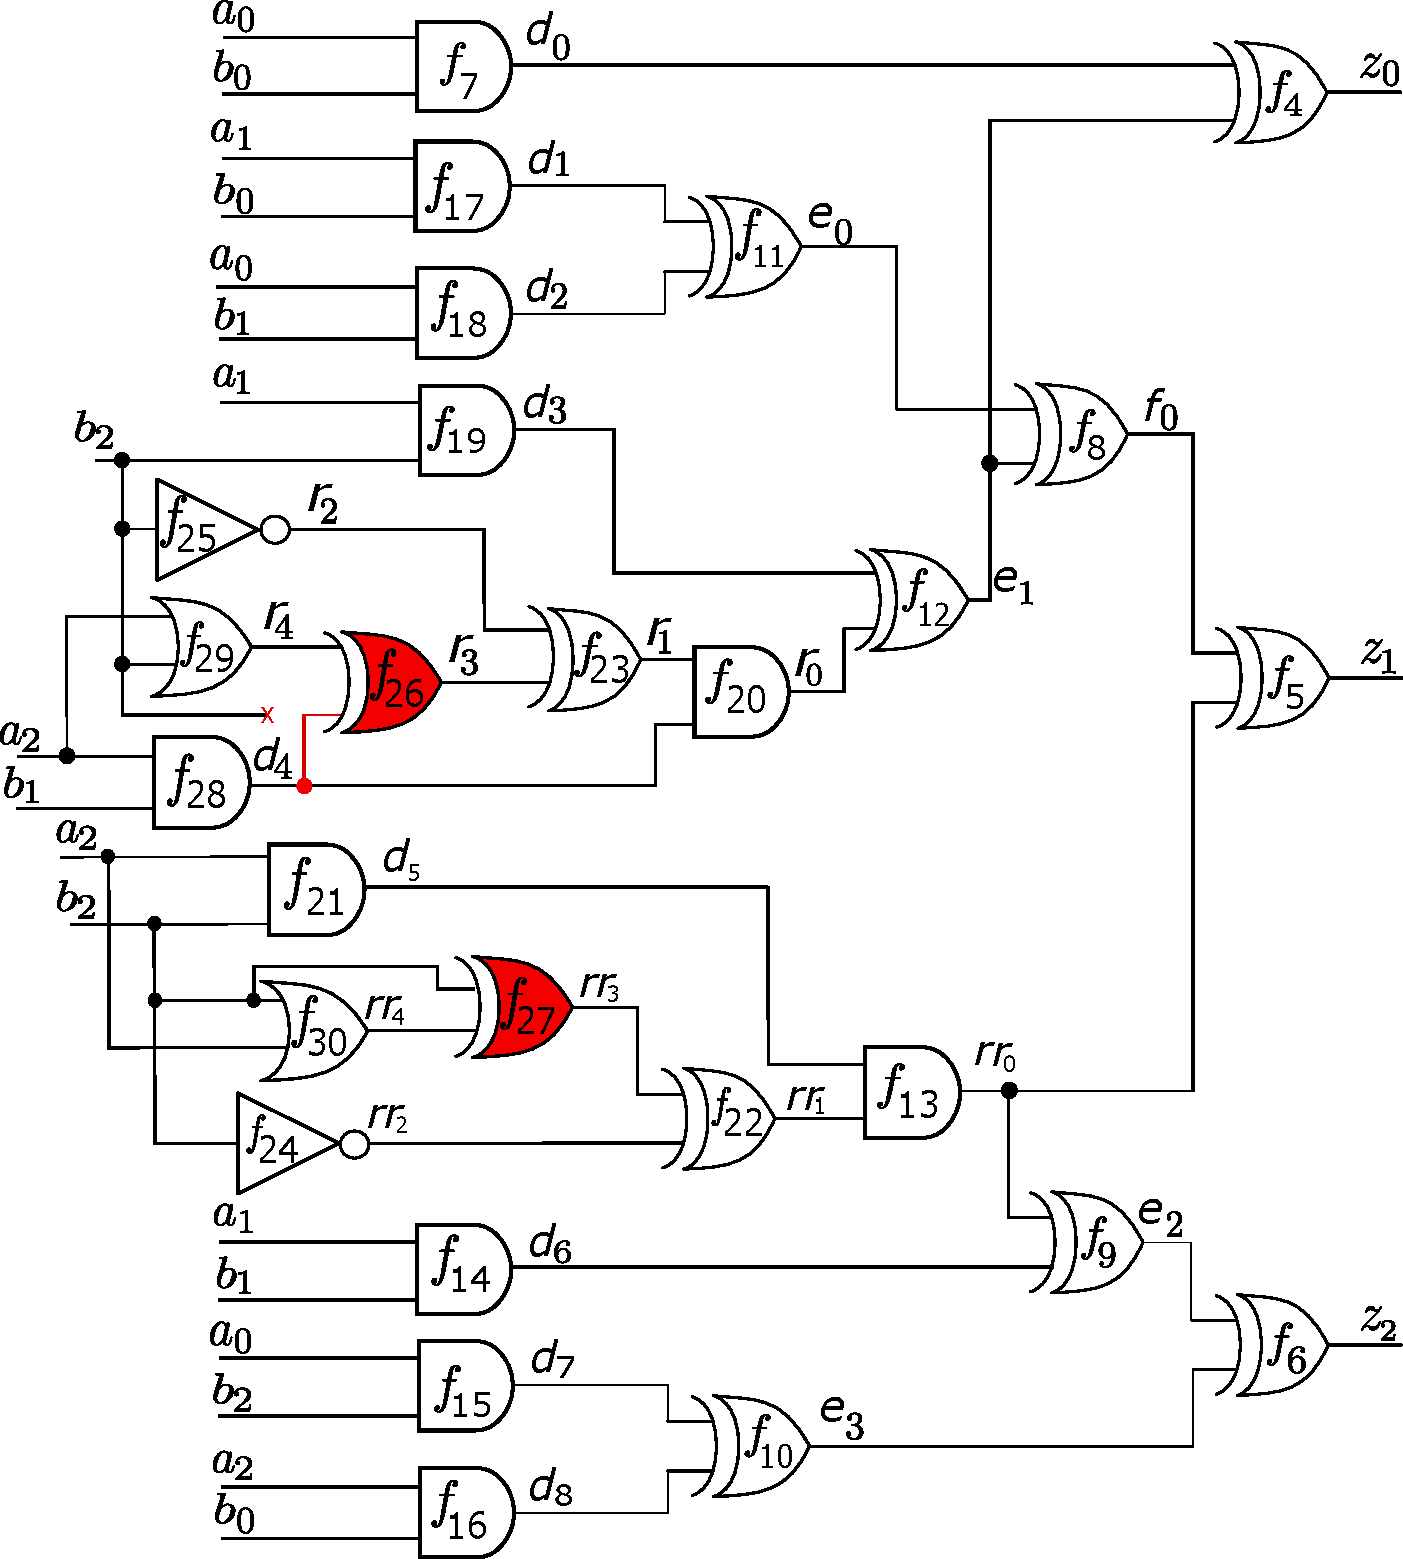
\includegraphics[scale=0.24]{mas_3_ddc_mfr_a.pdf}
% \caption*{A faulty implementation of a 3-bit ($n$=3) Mastrovito multiplier
% % ($n$=3) with gate replacement bugs introduced at nets $d_5$ (AND replaced with an OR) and $d_2$ (AND replaced with an XOR), and a wire replacement bug at net $e_0$ (input shorted to $d_0$ instead of $d_1$).
% }
% \end{figure}
% \end{frame}

% \begin{frame}{\large MFR Application: Polynomial modeling}
% \bi
% 	\item Denote polynomial $f: Z + A\cdot B$ as the design specification.
% 	\item Impose RTTO $>$
% \ei

% \begin{small}
% \begin{flalign*}
% f_1:Z + z_0 +\ga \cdot z_1 + \ga^2 \cdot z_2;   &\quad f_{22}:rr_1 + rr_3+rr_2; \\
% f_2:A + a_0 +\ga \cdot a_1 + \ga^2 \cdot a_2;   &\quad f_{23}:r_1 + r_2+r_3;\\
% f_3:B + b_0 +\ga \cdot b_1 + \ga^2 \cdot b_2;   &\quad \red{f_{26}:r_3 + r_4 + d_4;}\\
% f_4:z_0 + d_0 + e_1;                &\quad {\red f_{27}:rr_3 + rr_4 + b_2;}\\
% f_5:z_1 + f_0 + rr_0;               &\quad \dots\\
% \dots                               &\quad f_{30}:rr_4 + a_2+b_2+a_2b_2;
% \end{flalign*}
% \end{small}

% \bi
% \item $F = \{f_1,\dots,f_{30}\}$, $F_0 =\{a_0^2-a_0,\dots,z_2^2-z_2,A^8-A,\dots,Z^8-Z\}$. 
% %under RTTO $>$, $F\cup F_{0}$ constitutes a GB of
% \item Ideal $J+J_0=\langle F\cup F_0\rangle$ models $C$. 
% \ei
% \end{frame}

% \begin{frame}{\large MFR Notation: Field setup}
% \bi
% 	\item Circuit with data-path size $n$ modeled over $\Fkn$
% 	\bi
% 		% \item Polynomials modeled over $R=\Fkn[Z,A,x_1,\dots,x_d]$
% 		% \bi
% 		% 	\item $\{x_1, \dots$ $, x_d\}$ are all the bit-level variables (nets) in the circuit
% 		% 	\item $Z$ and $A$ are the word-level output and input, respectively
% 		% \ei
% 		\pause
% 		\item $\Fkn = \Ftwo[x]\pmod{P_n(x)}$
% 		\bi
% 			\item $P_n(x) \in \F_2[x]$ is a given degree-$n$ primitive polynomial; $P_n(\ga) =0$ 
% 			% [$\ga$ as one of its root].
% 		\ei
% 		\pause
% 		\item  Word-level polynomials for $Z,A$:
% 		\bi
% 			\item $f_Z: Z + \sum_{i=0}^{n-1}\ga^iz_i,~f_A: A + \sum_{i=0}^{n-1}\ga^ia_i$ 
% 		\ei
% 	\ei 
% 	\vspace{0.1in}
% 	\vspace{0.1in}
% 	\pause
% 	\item Patch size $m$ modeled over $\Fkm$
% 	\bi
% 		\pause
% 		\item $\Fkm = \Ftwo[x]\pmod{P_m(x)}$
% 		\bi
% 			\item We select a degree-$m$ primitive polynomial $P_m(x)\in \F_2[x]$; $P_m(\be) =0$ 
% 			% [$\be$ as one of its root].
% 		\ei
% 		\pause
% 		\item  Word-level polynomial for $W$:
% 		\bi
% 			\item $f_w: W + \sum_{i=0}^{m-1}\be^iw_i$
% 			\item $\{w_0,\dots,w_{m-1}\} \subset \{x_1,\dots,x_d\}$
% 		\ei
% 	\ei
% \ei
% \end{frame}

% \begin{frame}{\large Application: Word-level representation}
% \begin{figure}[hbt]
% \centering
%     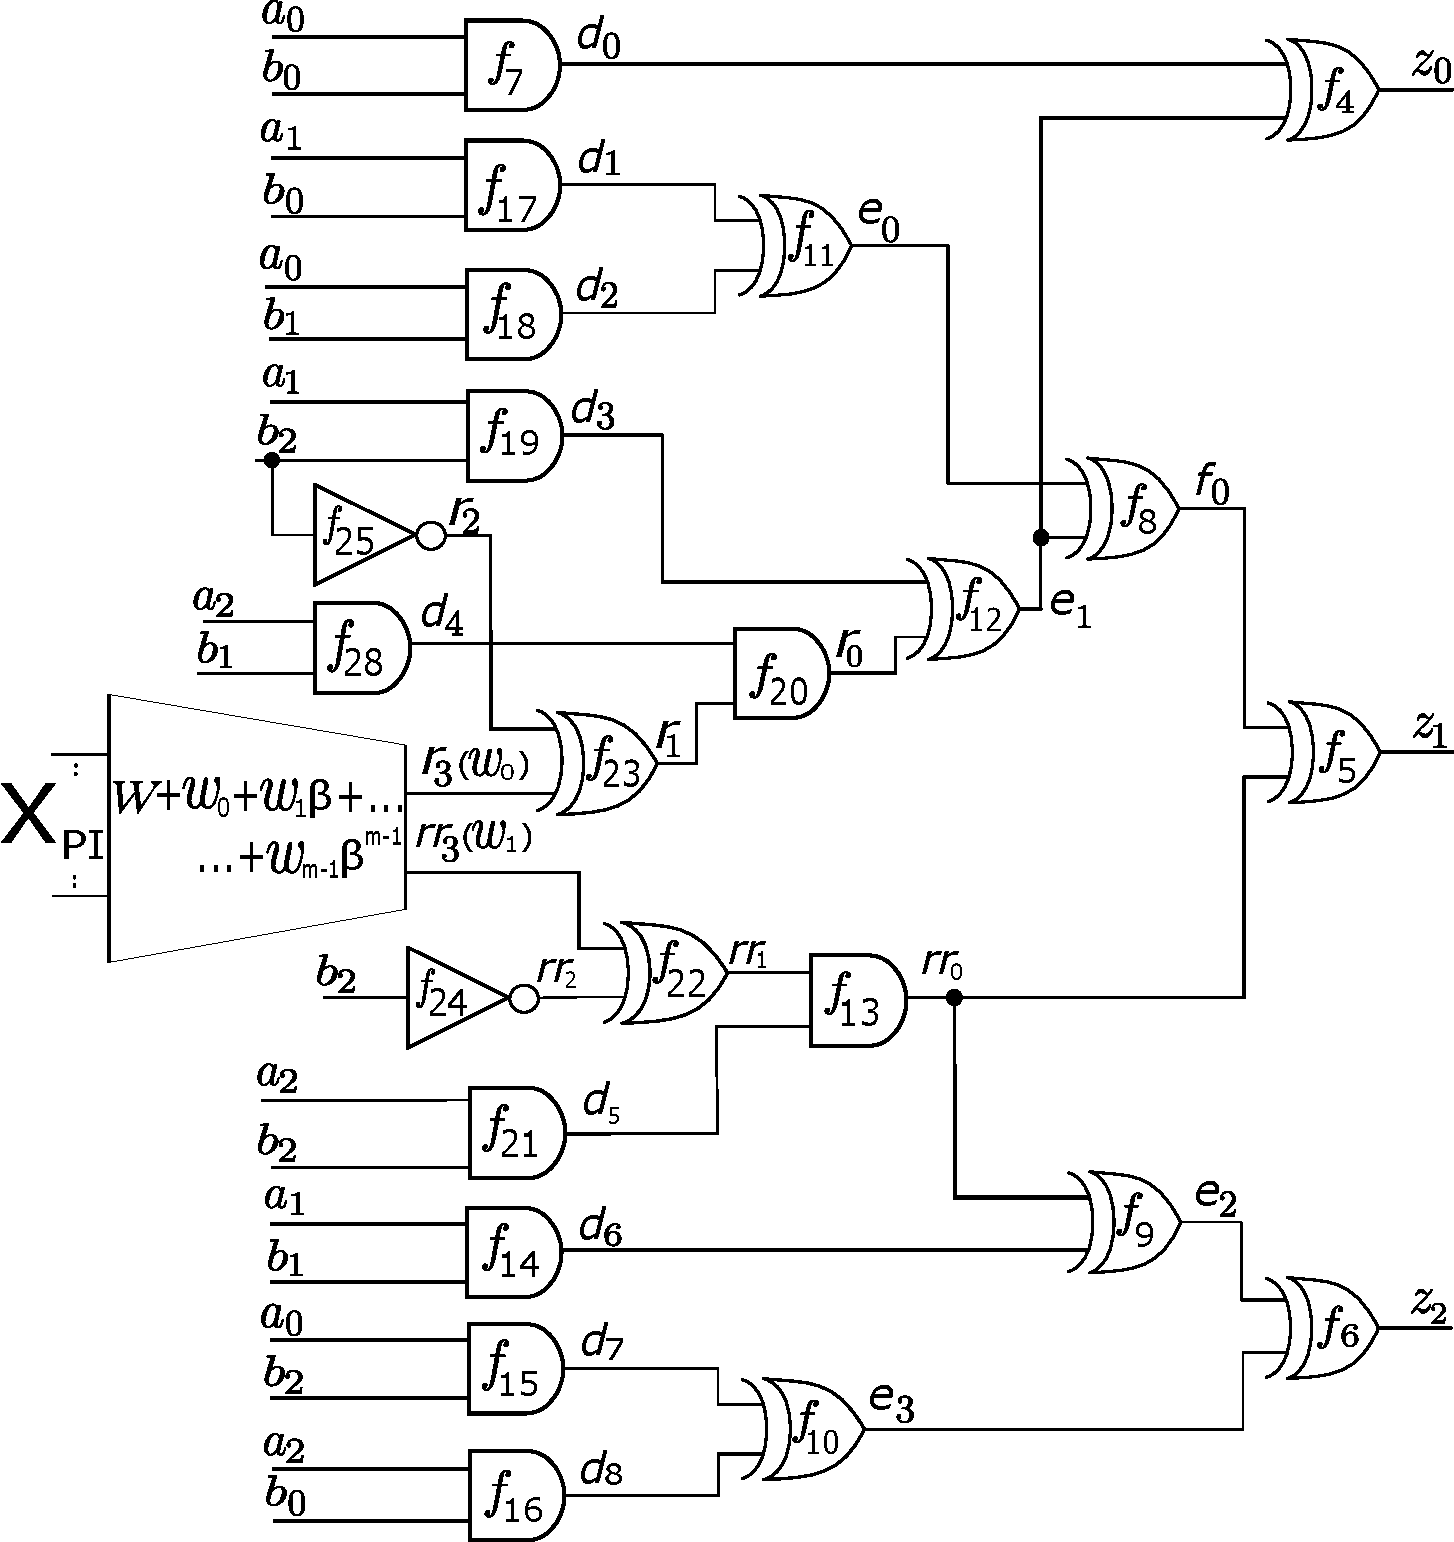
\includegraphics[scale = 0.24]{mas_3_ddc_mfr_b.pdf}
%     \caption*{
%     Patch function modeled as a 2-bit-vector word ($m$=2), 
%     $f_W: W+ r_3 + \beta \cdot rr_3$}
%     \label{fig:mas_bug_W_b}
% \end{figure}
% \end{frame}


% \begin{frame}{\large Mathematical Challenge: Picking $P_k(x)$}
% \bi 

% 	\item Need to represent and manipulate circuit polynomials and the patch function polynomials in one unified domain (composite field)
% 	% \bi
% 	% 	\item How to relate algebraic numbers of lower field to algebraic numbers of higher fields?
% 	% \ei
% 	\vspace{0.1in}
% 	\item Selecting arbitrary $P_k(x)$ leads to erroneous results 
% 	\vspace{0.1in}
% 	\item Solved using Univariate Polynomial Factorization

% \ei
% \end{frame}

\begin{frame}{\large MFR Challenges: $\Fkk$ and $P_k(x)$}
\bi
	% \item Determine the smallest single field ($\Fkk$) to operate both circuit ($\Fkn$) and patch ($\Fkm$)
	% \vspace{0.1in}
	% \item Composite field $\Fkk$ 
	% \bi
	% 	\item $\Fkm \subset \Fkk$ and $\Fkn \subset \Fkk$, $k=LCM(m,n)$
	% \pause
	% \vspace{0.1in}
	% \item What are the mathematical challenges?
	% \pause
	\item Smallest $k$ is $LCM(n,m)$
	\bi
		\vspace{0.1in}
		\item $\Fkk \supset \Fkn$ and $\Fkk \supset \Fkm$
		\vspace{0.1in}
		\item $\Fkk = \Ftwo[x]\pmod{P_k(x)}$
		\bi
			\item $P_k(x)$ is a degree-$k$ primitive polynomial; $P_k(\al) =0$ 
		\ei
	\ei
	\pause
	\vspace{0.1in}

	\item What $P_K(x)$ should be used for constructing $\Fkk$
	\vspace{0.1in}
	\pause
	\item  Mathematical challenge: Given $P_n(x)$ and $P_m(x)$, compute $P_k(x)$ such that
	$P_n(\ga)= P_m(\be)=P_k(\al)=0$
	\pause
	\bi
		\item How are elements $\al$, $\be$, and $\ga$ related?
	\ei
	\pause
	\item Solved using Univariate Polynomial Factorization and properties of finite fields
	\vspace{0.1in}
\ei

\end{frame}

% \begin{frame}{\large MFR Notations: Univariate Polynomial factorization (UPF) }
% \bi
% 	\item Given a monic univariate polynomial $f \in \F_q[X]$, where $\F_q$ is any finite field
% 	\vspace{0.1in}
% 	\bi 
% 		\item Find a complete factorization $f = f_1^{e_1}\cdot f_2^{e_2}\cdots f_l^{e_l}$ 
% 		\bi
% 			\item Where $f_1, f_2,\dots, f_l$ are pairwise distinct monic 
% 			irreducible polynomials in $\F_q[X]$ and $e_1,\dots,e_l$ are positive integers.
% 		\ei
% 	\ei
% 	\vspace{0.1in}
% 	% \item We employ existing implementation of UPF from computer algebra tool {\it SINGULAR} 
% \ei
% \end{frame}

% \begin{frame}{\large Contribution: Computing $P_k(x)$}
% \bi
% 	\vspace{0.1in}
% 	\item Property of finite fields, for any element $\phi \in \F_q$, $\phi^{q-1} = 1$
% 	\vspace{0.1in}
% 	\pause
% 	\bi
% 		\item $\ga = \al^{(2^k-1)/(2^n-1)} = \al^{\lambda}$
% 		\item $\be = \al^{(2^k-1)/(2^m-1)} = \al^{\mu}$
% 	\ei
% 	\pause
% 	\vspace{0.1in}
% 	\item Univariate Polynomial Factorization (UPF)
% 	\pause
% 	\vspace{0.1in}
% 	\bi
% 		\item Obtain UPFs of $P_n(x^{\lambda})$ and $P_m(x^{\mu})$ in $\F_2[x]$
% 	\ei
% 	% \bi
% 	% 	\item Coefficients will be in $\Ftwo$ and degrees will be less than $\lambda$ and $\mu$, respectively.
% 	% 	\bi
% 	% 		\item $P_n(x^{\lambda})=P_{n1}^{a1}\cdot P_{n2}^{a2}\cdots P_{nl}^{al}$, and 
% 	% 		\item $P_m(x^{\mu}) = P_{m1}^{b1}\cdot P_{m2}^{b2}\cdots P_{mg}^{bg}$
% 	% 	\ei
% 	% \ei
% 	\pause
% 	\vspace{0.1in}
% 	\item Then, $\exists P_{k}(x) \in \F_2[x]$ as a common factor of $P_n(x^{\lambda})$ and $P_m(x^{\mu})$, such that:
% 	\bi
% 		\item $P_{k}(x)$ is a degree-$k$ primitive polynomial in $\F_2[x]$ with $P_k(\al)=0$
% 	\ei
% \ei
% \end{frame}

\begin{frame}{\large Application: Word-level representation}
\begin{figure}[hbt]
\centering
    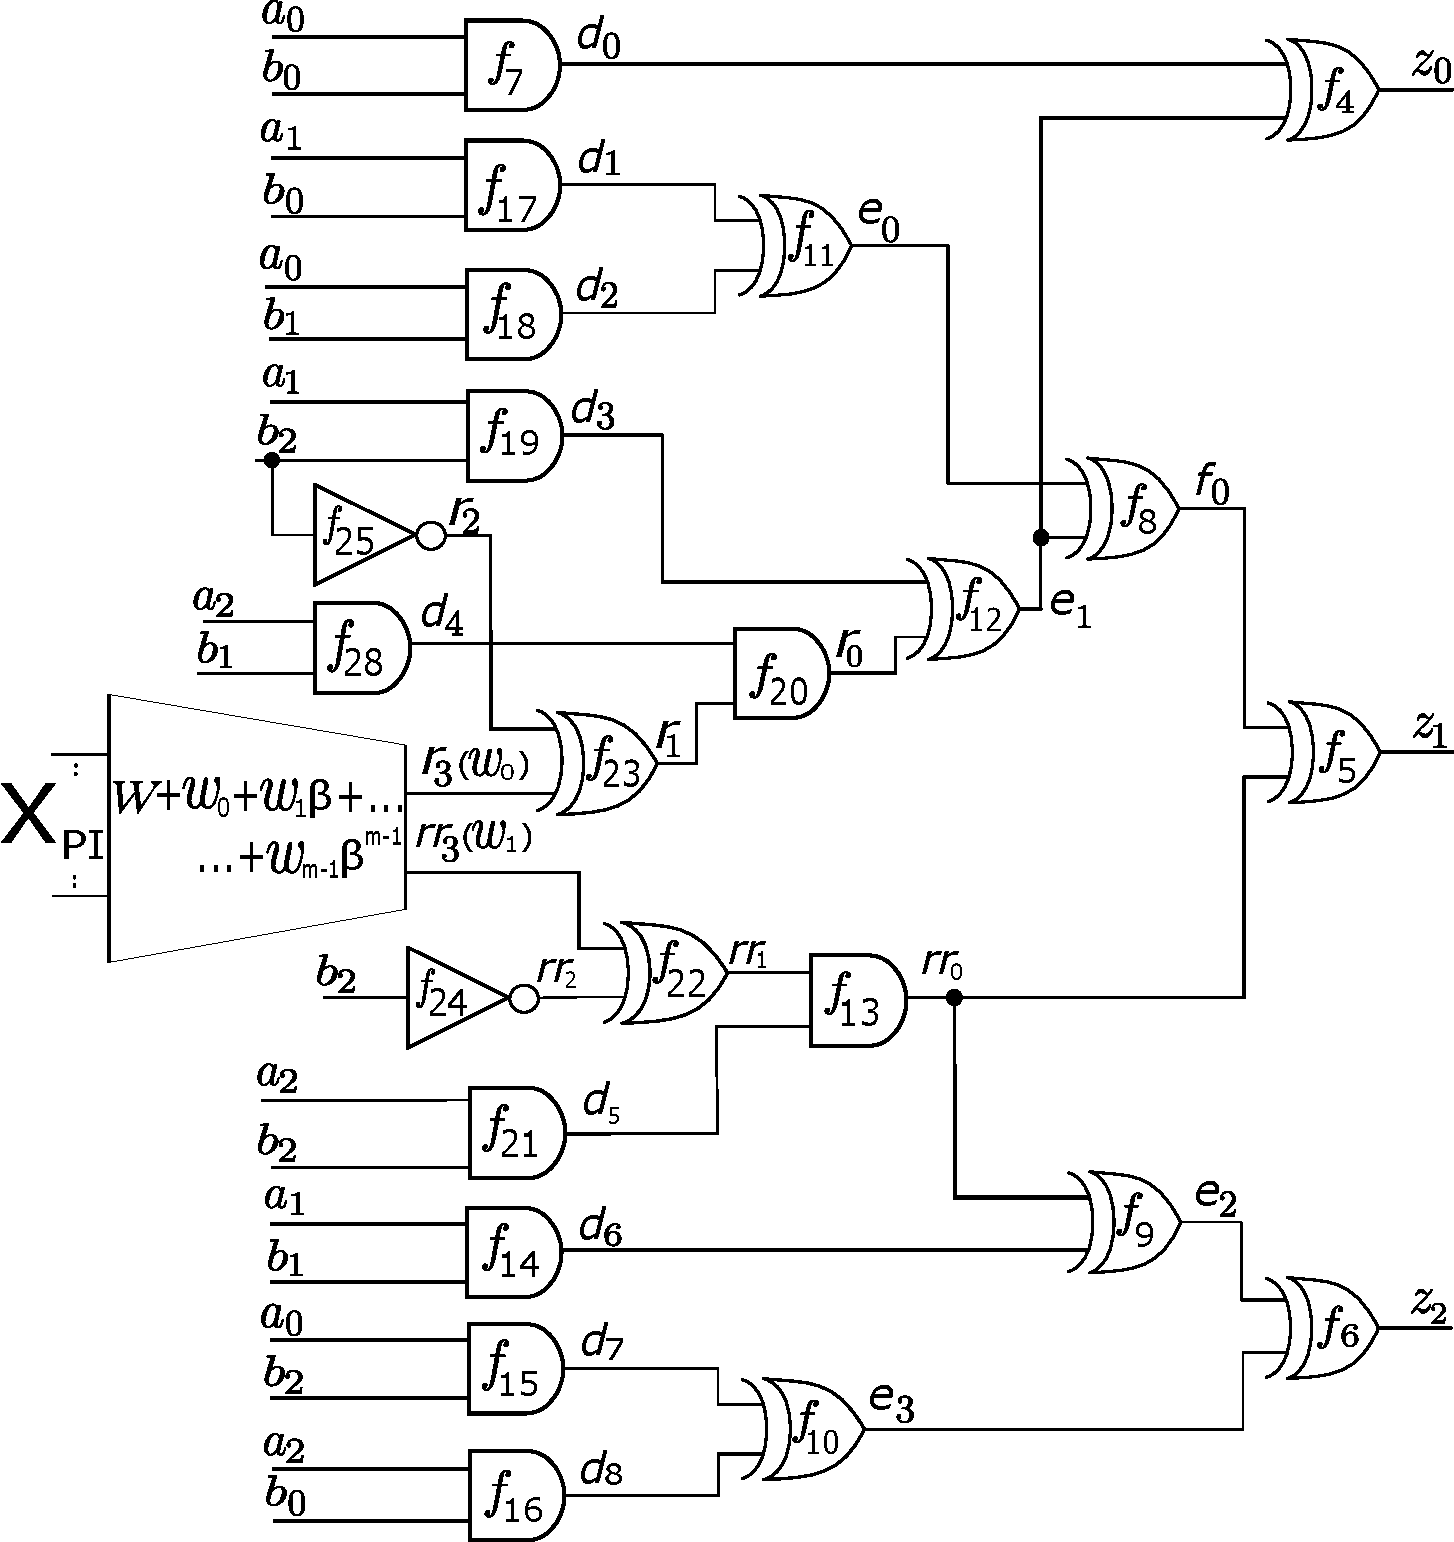
\includegraphics[scale = 0.24]{mas_3_ddc_mfr_b.pdf}
    \caption*{
    Patch function modeled as a 2-bit-vector word ($m$=2), 
    $f_W: W+ r_3 + \beta \cdot rr_3$}
\end{figure}
\end{frame}

% \begin{frame}{\large Application: Computing $P_k(x)$}
% \bi
% \item $P_3(x) = x^3+x+1,~~P_2(x) = x^2+x+1,~~\ga = \al^9,~~\be=\alpha^{21}$
% \pause
% \vspace{0.1in}
% 	\item Composite field: $k=LCM(2,3)=6$
% 	\vspace{0.1in}
% 	\pause
% 	\bi
% 		\item $ UPF(P_3(x^9)) = (x^9)^3+(x^9)+1 =
%   \textcolor{red}{(x^6+x^5+x^2+x+1)}\textcolor{green}{(x^6+x^5+1)}\textcolor{green}{(x^6+x^4+x^3+x+1)}(x^6+x^4+x^2+x+1)(x^3+x+1);$
% 		\vspace{0.1in}
% 		\pause
% 		\item $UPF(P_2(x^{21})) = (x^{21})^2+(x^{21})+1 =
%   \textcolor{red}{(x^6+x^5+x^2+x+1)}\textcolor{green}{(x^6+x^5+1)}\textcolor{green}{(x^6+x^4+x^3+x+1)}(x^6+x^5+x^3+x^2+1)
%   (x^6+x^5+x^4+x+1)(x^6+x+1)(x^6+x^3+1);$
% 		% \pause
% 		% \vspace{0.1in}
% 		% \item We choose $P_6(x)=x^6+x^5+1$ as the required $P_k(x)$.
% 	\ei
% \ei
% \end{frame}

% \begin{frame}{\large Circuit polynomials over $\Fkk$}
% \bi
% 	\item Boolean logic gates in $\F_2 ~~(\F_2 \subset \Fkk)$. Over $\F_2$, $-1=+1\pmod{2}$
% \ei
% 	\begin{align*}
% 		 z &=~ \sim a &\implies &z+a+1 &\pmod{2}\\
% 		 z &= a \wedge b &\implies &z+a\cdot b &\pmod{2}\\
% 		 z &= a \vee b &\implies &z+a\cdot b + a + b &\pmod{2}\\
% 		 z &= a \oplus b &\implies &z+a+b &\pmod{2}
% 	\end{align*}
% \pause
% \bi
% 	\item Word-level polynomials with $\ga = \al^{\lambda}$ and $\be = \al^{\mu}$
% 	% \bi 
% 		% \item $\ga$ = primitive element of $\Fkn$, i.e. $P_n(\ga)=0$
% 	% \ei
% \ei
% \begin{equation*}
% \begin{split}
%  Output:& Z + z_0 +\gamma \cdot  z_1 + \dots +\gamma^{n-1} \cdot z_{n-1}\\
%  Input: & A + a_0 +\gamma \cdot a_1 + \dots +\gamma^{n-1} \cdot a_{n-1} \\
%  Patch: & W + w_0 +\beta \cdot w_1 + \dots +\beta^{m-1} \cdot w_{m-1}
% \end{split}
% \end{equation*}
% \end{frame}

\begin{frame}{\large Circuit Polynomials and Setup}
\bi
	\item Ring $R = \Fkk[Z,A,B,\dots,W,r_3,rr_3,\dots,a_0,a_1,\dots,b_1,b_2]$ 
	\vspace{0.1in}
	\pause
	\item Circuit polynomials under a term order $>$:
	\begin{small}
	\begin{flalign*}
	f_1:Z + z_0 +\ga \cdot z_1 + \ga^2 \cdot z_2;   &\quad f_{22}:rr_1 + rr_3+rr_2; \\
	f_2:A + a_0 +\ga \cdot a_1 + \ga^2 \cdot a_2;   &\quad f_{23}:r_1 + r_2+r_3;\\
	f_3:B + b_0 +\ga \cdot b_1 + \ga^2 \cdot b_2;   &\quad \red{f_{26}:r_3 + r_4 + d_4;}\\
	f_4:z_0 + d_0 + e_1;                &\quad {\red f_{27}:rr_3 + rr_4 + b_2;}\\
	f_5:z_1 + f_0 + rr_0;               &\quad \dots\\
	\dots                               &\quad f_{30}:rr_4 + a_2+b_2+a_2b_2; \\
	\dots								&\quad f_W:W + r_3 + \be \cdot rr_3;
	\end{flalign*}
	\end{small}
	\vspace{-0.2in}
	\pause
	\item $F = \{f_1,\dots,f_{30},f_W\}$
	\item $F_0 =\{a_0^2-a_0,\dots,z_2^2-z_2,A^8-A,\dots,Z^8-Z,W^4-W\}$. 
	% \bi
	% 	\item Ideal $J+J_0=\langle F\cup F_0\rangle$ models $C$.
	% \ei
\ei

\end{frame}
% \begin{frame}{\large MFR Notation: Incorrect $P_k(x)$}
% \bi
% 	\item If we incorrectly choose $P_k(x)=x^6+x^3+1$
% 	\pause
% 	\item For its root $\al$, we have
% 	\pause
% 	\begin{align*}
% 	\alpha^6 + \alpha^3 + 1 &= 0\\
%  	(\alpha^3)(\alpha^6 +\alpha^3 + 1) &= 0 ~(\text{multiply by}~\alpha^3)\\
% 	\alpha^9 + \alpha^6 + \alpha^3 &= 0 \\
% 	\gamma + 1 &= 0
% % \stepcounter{equation}\tag{\theequation}\label{ll} 
% \end{align*}
% 	\pause
% 	\item However, $\ga \neq 1$, as $\ga$ is a primitive element of $\Fkn$
% 	\item Selecting arbitrary $P_k(x)$ leads to erroneous results
% \ei
% \end{frame}

% \begin{frame}{\large Application: Word-level representation}
% \begin{figure}[hbt]
% \centering
%     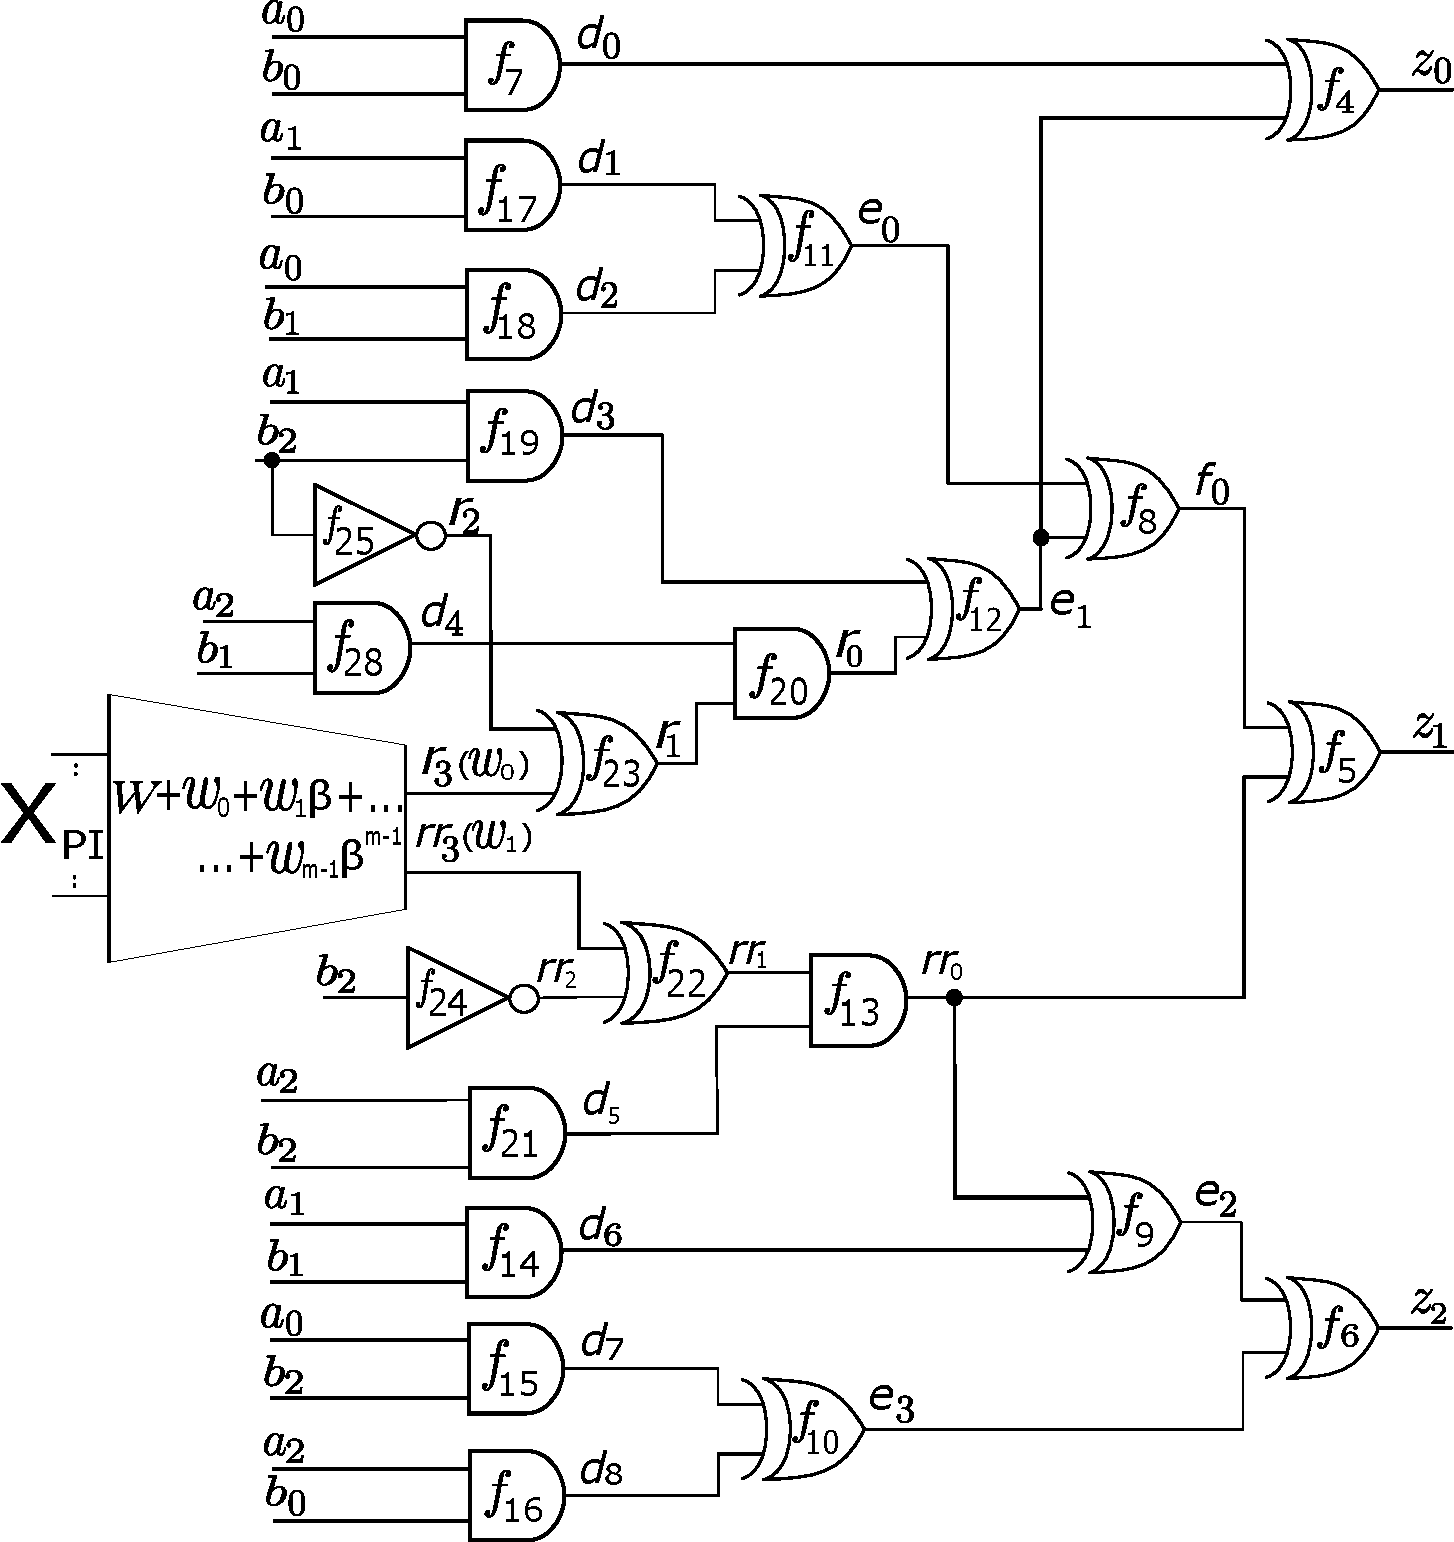
\includegraphics[scale = 0.24]{mas_3_ddc_mfr_b.pdf}
%     \caption*{
%     Patch function modeled as a 2-bit-vector word ($m$=2), 
%     $f_W: W+ r_3 + \beta \cdot rr_3$}
% \end{figure}
% \end{frame}


% \begin{frame}{\large MFR Notation: Word-level reasoning}
% \bi
% 	\item Obtain each $w_i$ as a polynomial function in $W,\beta$
% 	\bi
% 		\item $\forall i \in 1,\dots,m,~~w_i= \mathcal{F}_i(W,\beta)$
% 	\ei
% 	\pause
% 	\begin{align*}
% 	W & = w_0 + \dots + \beta^{m-1} \cdot w_{m-1}\\
%     W^2 & = w_0^2 + \dots + \beta^{2(m-1)}\cdot w_{m-1}^2\\
%         & \dots \\
%     W^{2^{m-1}} & = w_0 + \dots + \beta^{2^{m-1}(m-1)}\cdot w_{m-1}
%     \end{align*}
% 	\pause
% 	\item Solved using Gaussian elimination
% \ei
% \end{frame}

% \begin{frame}{\large MFR Notation: MFR setup steps}
% \begin{enumerate}
% 	\item Setup a new ring $R' = \Fkk[x_1,\dots,x_d,Z,A,W]$ 
% 	\bi
% 		\item $\Fkk$ is constructed using $P_k(x)$
% 		\item Modify RTTO $>$ to place the target $W$ before the lowest indexed target $w_i$
% 	\ei
% 	\vspace{0.1in}
% 	\pause
% 	\item Construct a polynomial set $F'$ as follows:
% 	\bi
% 		\pause
% 		\item Start with $F' = F$
% 		\pause
% 		\item Remove polynomials with $w_i$'s as leading terms
% 		\pause
% 		\item Substitute $\forall i \in 1,\dots,m,~~w_i= \mathcal{F}_i(W,\beta)$
% 		\pause
% 		\item Add $f_w: W + \sum_{i=0}^{m-1}\be^iw_i$
% 		\pause
% 		\item Substitute $\beta = \alpha^{\mu}, \gamma=\alpha^{\lambda}$
% 	\ei

% \end{enumerate}
% \end{frame}


% \begin{frame}{\large Circuit Polynomials and Setup}
% \bi
% 	\item Ring $R = \Fkn[x_1,\dots,x_d,Z,A]$ 
% 	\bi
% 		\item $\Fkn$ is constructed using $P_n(x)$
% 	\ei
% 	\item Circuit polynomials under RTTO $>$:
% 	\begin{small}
% 	\begin{flalign*}
% 	f_1:Z + z_0 +\ga \cdot z_1 + \ga^2 \cdot z_2;   &\quad f_{22}:rr_1 + rr_3+rr_2; \\
% 	f_2:A + a_0 +\ga \cdot a_1 + \ga^2 \cdot a_2;   &\quad f_{23}:r_1 + r_2+r_3;\\
% 	f_3:B + b_0 +\ga \cdot b_1 + \ga^2 \cdot b_2;   &\quad \red{f_{26}:r_3 + r_4 + d_4;}\\
% 	f_4:z_0 + d_0 + e_1;                &\quad {\red f_{27}:rr_3 + rr_4 + b_2;}\\
% 	f_5:z_1 + f_0 + rr_0;               &\quad \dots\\
% 	\dots                               &\quad f_{30}:rr_4 + a_2+b_2+a_2b_2;
% 	\end{flalign*}
% 	\end{small}
% 	\vspace{-0.1in}
% 	\item $F = \{f_1,\dots,f_{30}\}$, $F_0 =\{a_0^2-a_0,\dots,z_2^2-z_2,A^8-A,\dots,Z^8-Z\}$. 
% 	\bi
% 		\item Ideal $J+J_0=\langle F\cup F_0\rangle$ models $C$.
% 	\ei
% \ei

% \end{frame}

% \begin{frame}{\large MFR Application: Word-level Formulation }
% \bi
% 	\item ring $R' = \F_{2^6}[x_1,\dots,x_d,Z,A,W]$ 
% 	\bi
% 		\item $\F_{2^6} = \F_2[x]$ (mod $P_6(x)$), $P_6(x) = x^6+x^5+1$
% 		\pause 
% 		\vspace{0.1in}
% 		\item WRTO $>$: {\small 
% $\{Z\}>\{A>B\}>\{z_0>z_1>z_2\}>\cdots>\{d_1>d_2>d_3>r_0>d_5>rr_1\}>
% \{r_1\}>{\bf \{W\}}>\{{\bf rr_3}>rr_2\}>\{r_2>{\bf r_3}>rr_4\}>\{r_4>d_4\}>\{a_0>a_1>a_2>b_0>b_1>b_2\}$}

% 	\ei
% 	\vspace{0.1in}
% 	\pause
% 	\item Update polynomial set $F$ to $F'$ as:
% 	\begin{align*}
% 		&rr_3= W^2+W,~~r_3 = \be W^2 +\be^2W \\
% 		&f'_{22}:rr_1  + (W^2+W) + rr_2\\
% 		&f'_{23}:r_1 + r_2 + (\be W^2 +\be^2 W)\\
% 		&f_W:W + r_3 + \be \cdot rr_3\\     
% 		&\be=\al^{21} \text{ and } \ga=\al^9 \\
% 		&F'=\{f_1,\dots,f_{21},~f'_{22},f'_{23},f_W,\dots,f_{30}\}-\{f_{26},f_{27}\}
% 	\end{align*}
% \ei
% \end{frame}

% \begin{frame}{\large MFR Contribution: Rectification Check}
% %ATPG V() V() = empty
% %we have an algebraic proof which is there in the proposal
% \bi
% 	\item Multi-fix rectification at target $W$
% 	\vspace{0.1in}
% 	\bi
% 		\item Construct the following polynomial sets:
% 		\begin{align*}
% 			F_l' =\langle f_1,\dots,f_W=W+\delta[l],\dots,f_s\rangle,1 \leq l \leq 2^m, \\
% 			% \text{ where $F_l'$ is obtained from $F'$ by replacing } \\
% 			% f_W \in F' \text{ with } f'_W: W + \delta[l], 1\leq l \leq 2^m,\text{ and } \\
%   			Where~(\delta[1],\dots,\delta[2^{m}]) =(0,1,\be,\dots,\be^{2^m-2}).
% 		\end{align*}
% 		\pause
% 		\item Reduce the specification $f: Z+A\cdot B$ modulo these sets: 
% 		\bi
% 			\item $f\xrightarrow{F_l', F_0}_+rem_l $, $\forall 1 \leq l \leq 2^m$
% 		\ei
% 		% \item Let $V_{\Fq}(rem_l)$ denote the varieties of the respective $rem_l$'s
% 		\vspace{0.2in}
% 		\pause
% 		\item Multi-fix rectification exists at target $W$: \\  
% 				\centering
% 				{\bf if and only if} $ \prod_{l=1}^{2^m} rem_l \xrightarrow{F_0}_+0$
% 	\ei
% \ei
% \end{frame}
\begin{frame}{\large Contribution: Multi-fix Rectification Check}
\bi
	\item Constructing the $F'_l$:
	\bi
		\item {$F_1'$, where $F_1'[f_W]=W+0$},
		\item {$F_2'$, where $F_2'[f_W]=W+1$},
		\item {$F_3'$, where $F_3'[f_W]=W+\be$},
		\item {$F_4'$, where $F_4'[f_W]=W+\be^2$}
	\ei
	\vspace{0.1in}
	\pause
	\item Reducing the specification $f: Z+A\cdot B$:
\bi
\item $rem_1 = f \xrightarrow[]{F_1'\cup F_{0}}_+{\al^{27} (a_2b_1b_2)+\al^{36} (a_2b_2)}$
\item $rem_2 = f \xrightarrow[]{F_2'\cup F_{0}}_+{\al^{27} (a_2b_1b_2+a_2b_1)+\al^{36} (a_2b_2)}$
\item $rem_3 = f \xrightarrow[]{F_3'\cup F_{0}}_+{\al^{27} (a_2b_1b_2)}$
\item $rem_4 = f \xrightarrow[]{F_4'\cup F_{0}}_+{\al^{27} (a_2b_1b_2+a_2b_1)}$
\ei \pause
	\item $rem_1\cdot rem_2 \cdot rem_3 \cdot rem_4 \xrightarrow{F_0}_+0$
	\item Target $W$ with nets $r_3$ and $rr_3$ admits MFR
\ei
\end{frame}


\begin{frame}{\large Rectification check: Remainder generation}
\begin{figure}[hbt]
\centering
    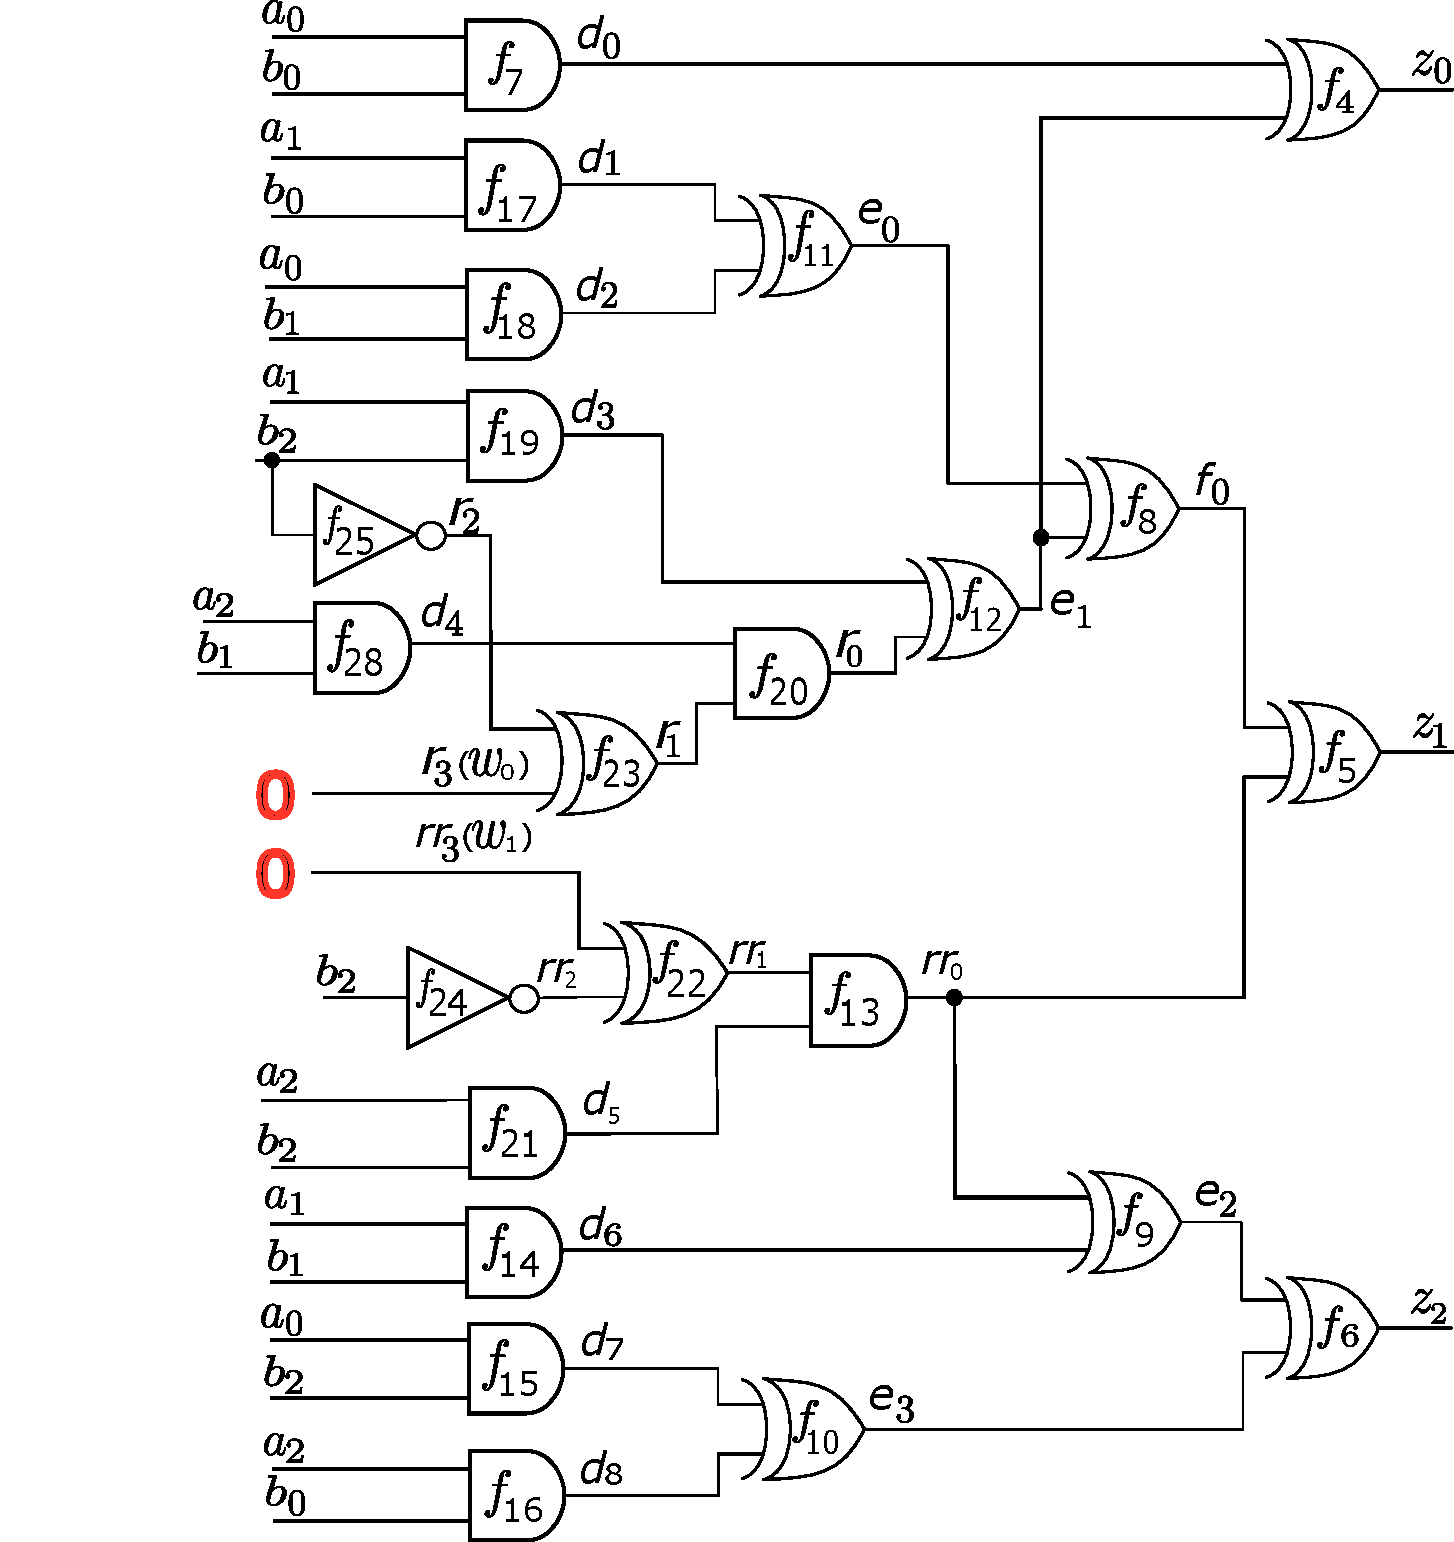
\includegraphics[scale = 0.28]{mas_3_ddc_mfr_b_00.pdf}
    \caption*{}
\end{figure}
\end{frame}

\begin{frame}{\large Rectification check: Remainder generation}
\begin{figure}[hbt]
\centering
    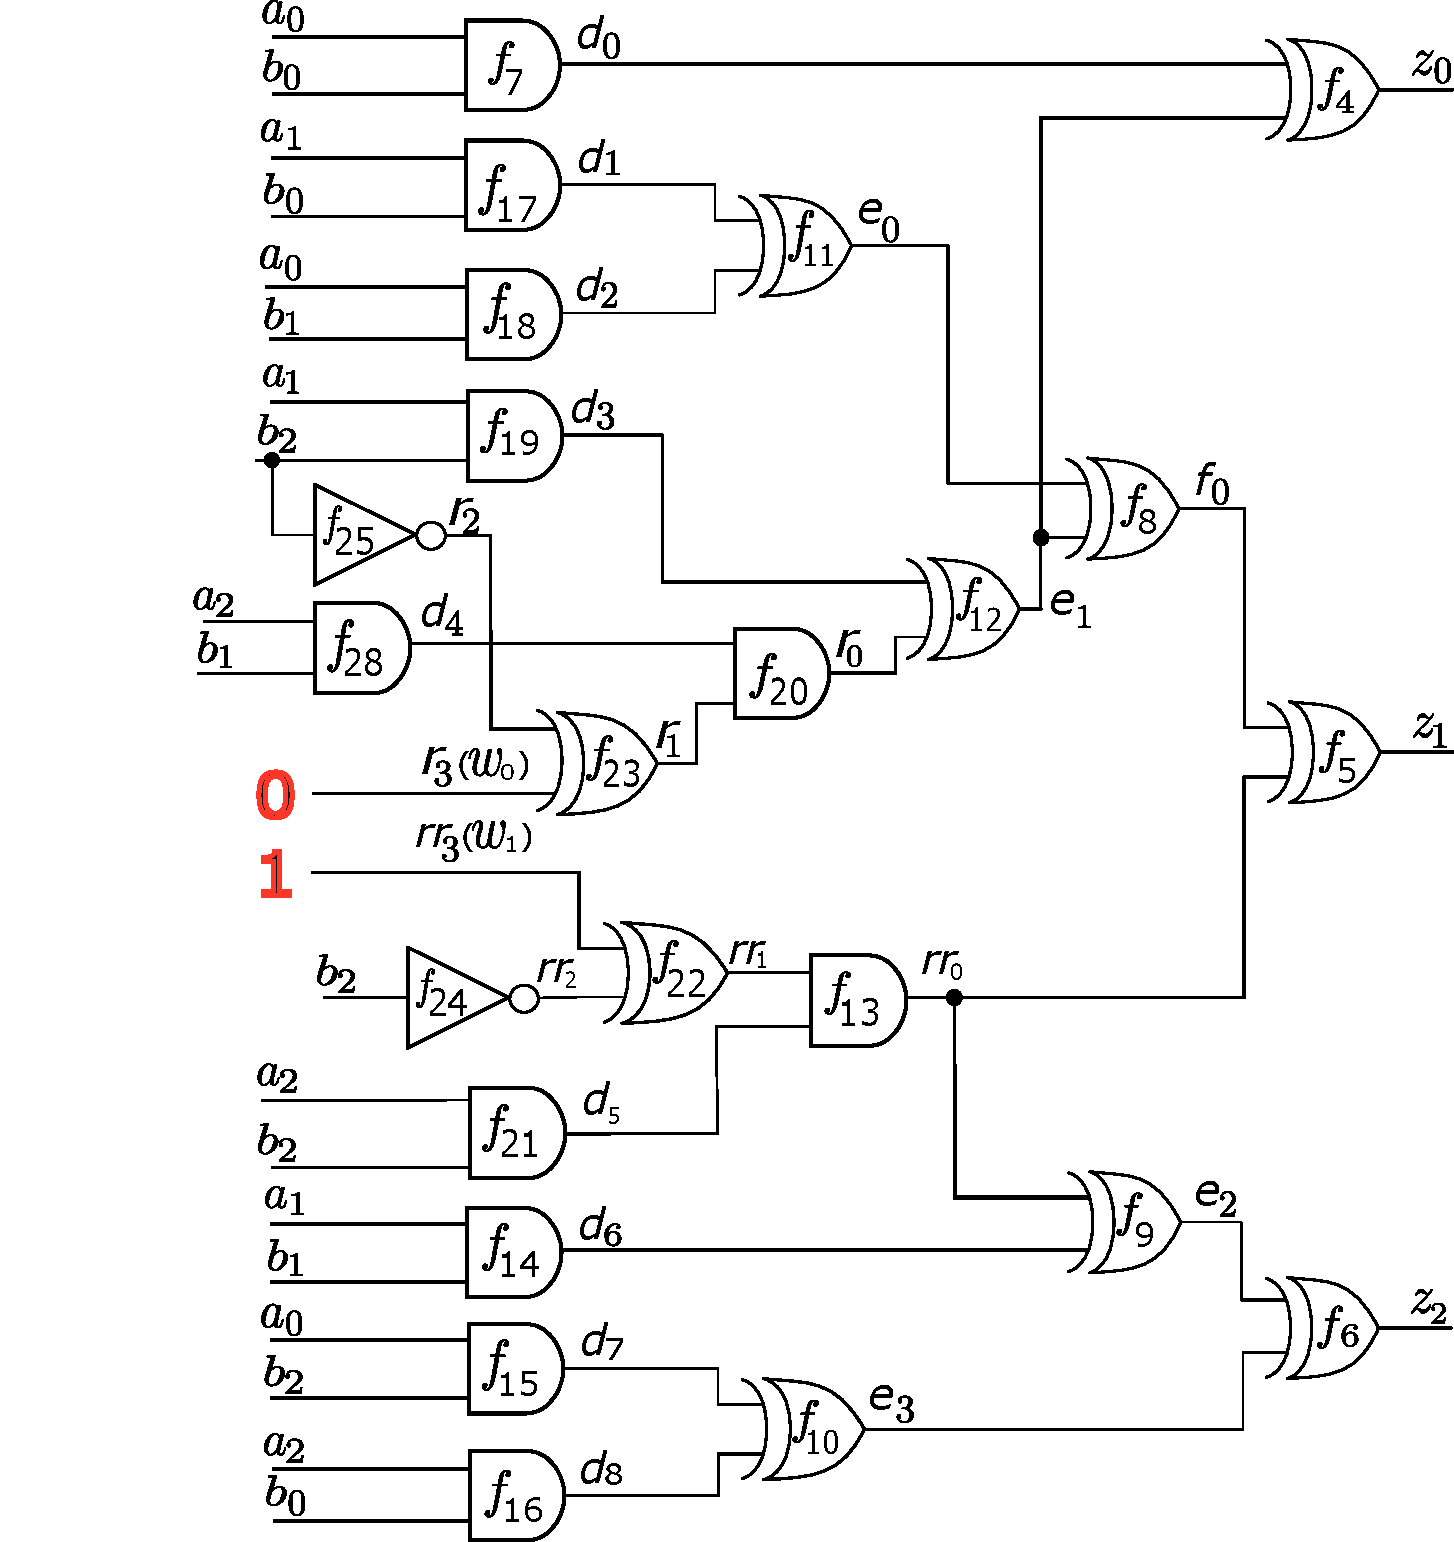
\includegraphics[scale = 0.28]{mas_3_ddc_mfr_b_10.pdf}
    \caption*{}
\end{figure}
\end{frame}

\begin{frame}{\large Rectification check: Remainder generation}
\begin{figure}[hbt]
\centering
    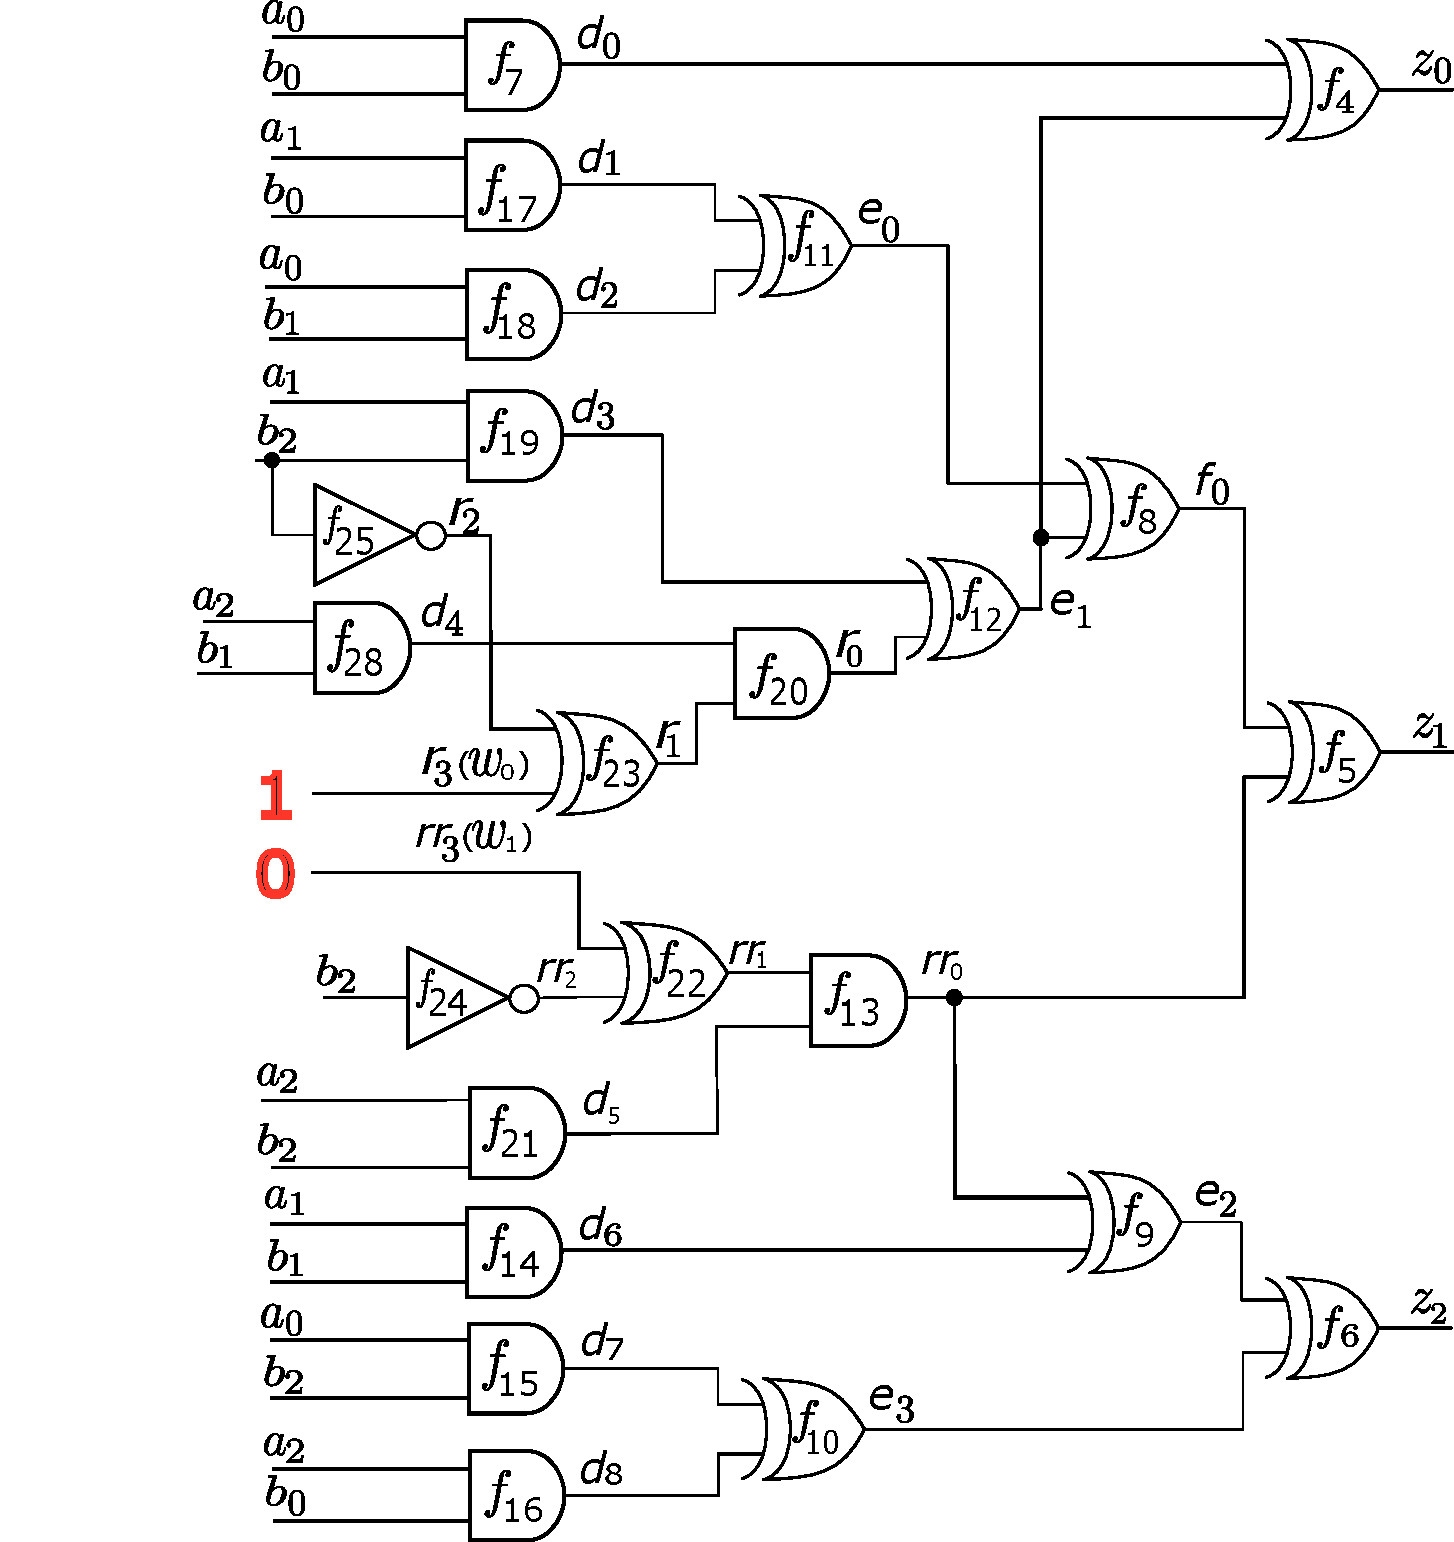
\includegraphics[scale = 0.28]{mas_3_ddc_mfr_b_01.pdf}
    \caption*{}
\end{figure}
\end{frame}

\begin{frame}{\large Rectification check: Remainder generation}
\begin{figure}[hbt]
\centering
    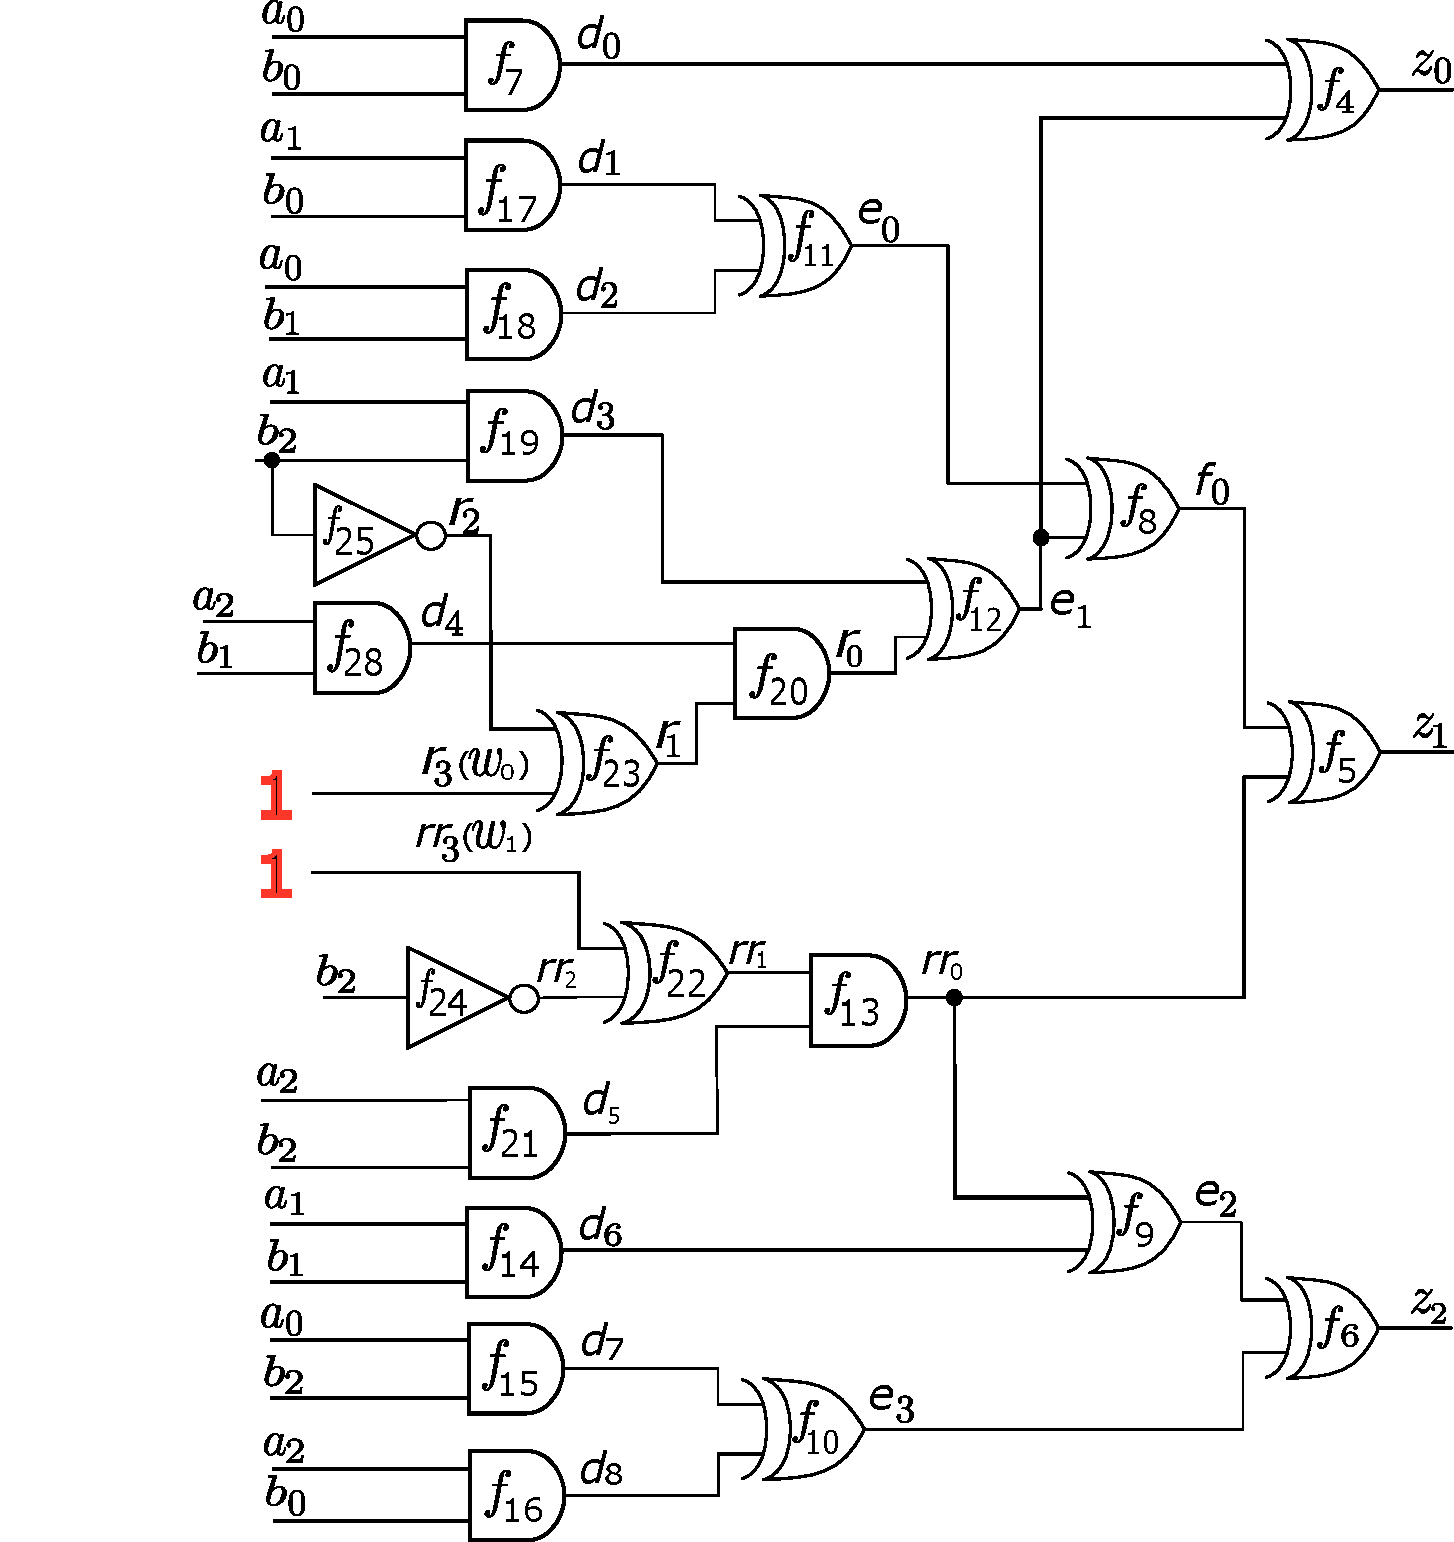
\includegraphics[scale = 0.28]{mas_3_ddc_mfr_b_11.pdf}
    \caption*{}
\end{figure}
\end{frame}


% \begin{frame}{\large Future work: Rectification function}

% \bi
% \item A polynomial which can be computed to rectify the circuit
% 	\bi
% 		\item $W = a_2b_1b_2 + \beta \cdot a_2b_2$
% 		\item $r_3 = (a_2 \wedge b_1 \wedge b_2),~~rr_3 = (a_2 \wedge b_2)$
% 	\ei
% \ei

% \end{frame}

% \begin{frame}{\large MFR Pseudocode}
% \begin{figure}[hbt]
% \centering
%     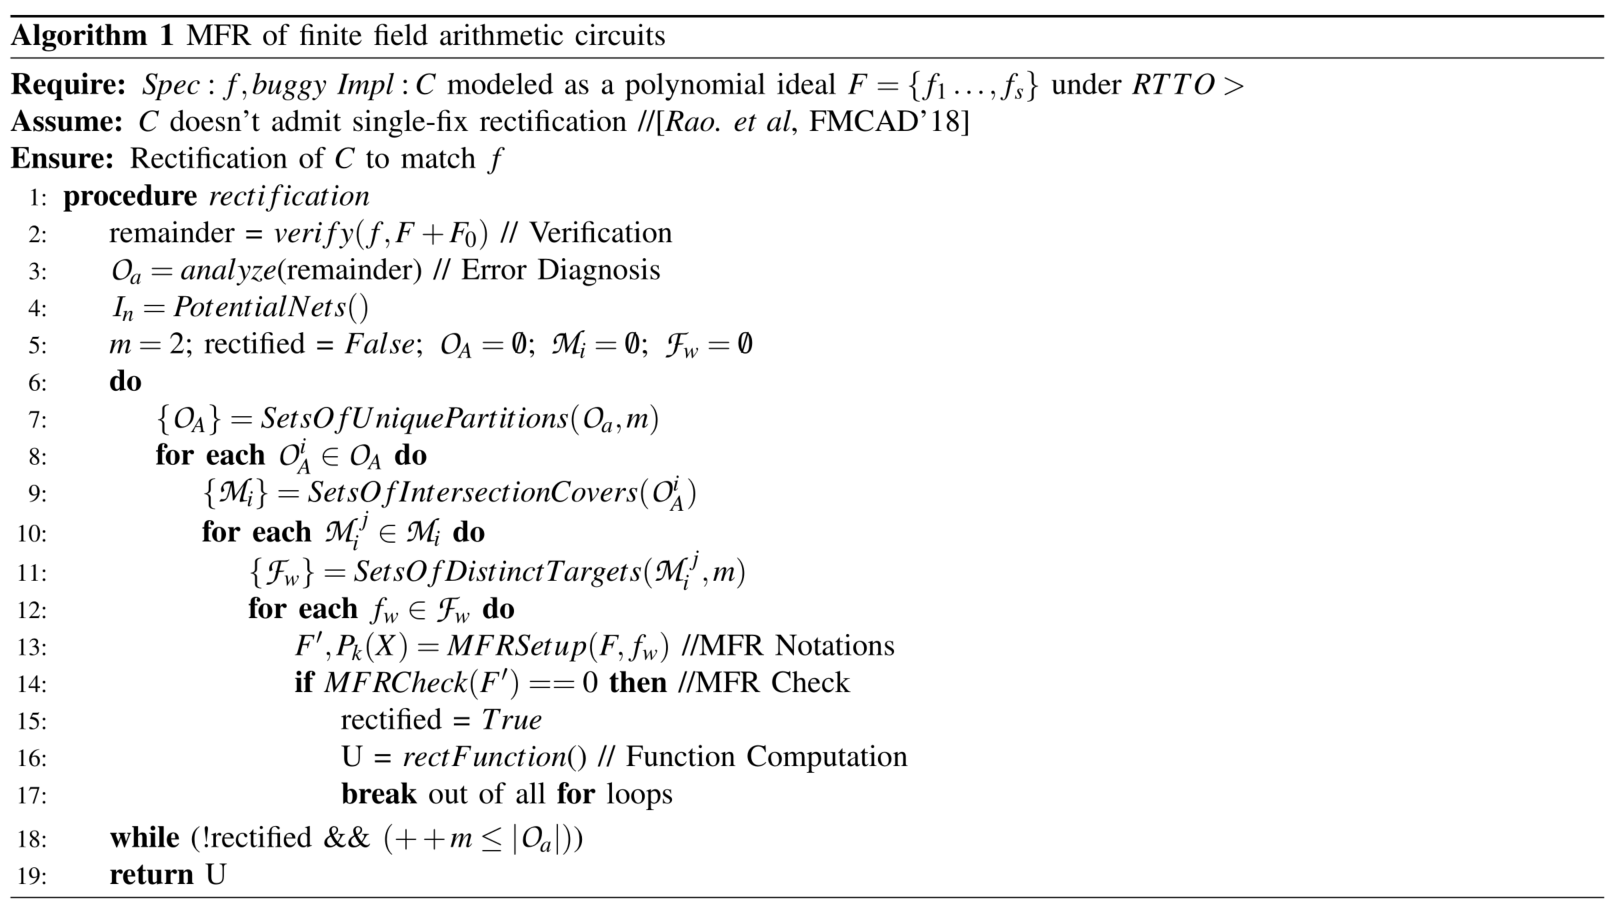
\includegraphics[scale = 0.43]{algo.png}
% \end{figure}
% \end{frame}

% \begin{frame}{\large Research Objective: Synthesis of Rectification Function}
% \begin{figure}[hbt]
%     \begin{center}
%     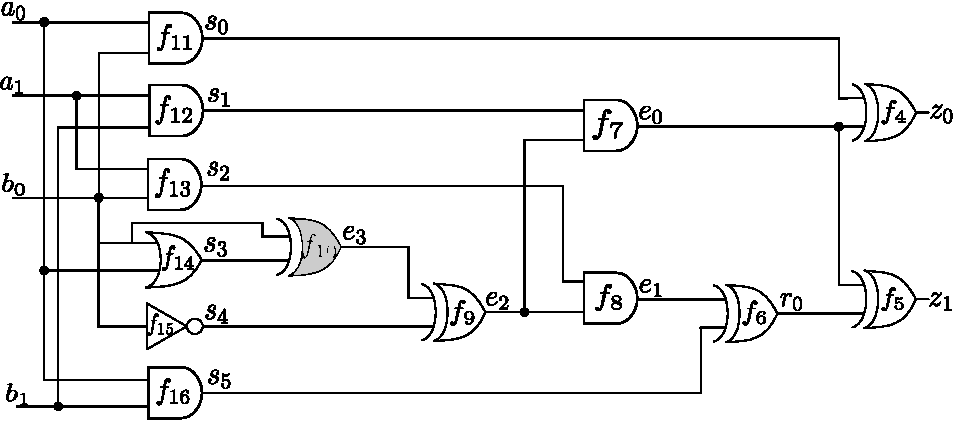
\includegraphics[scale = 0.7]{mas_red_bug-eps-converted-to.pdf}
%     \end{center}
% %    \vspace{-4ex}
%     \caption*{\small A 2-bit buggy modulo
%       multiplier implementation. 
%     %   with the bug at
%     % net $e_3$. A correct implementation will have an AND gate at $e_3$,
%     % which has been replaced by an XOR gate.
%     }
%     \label{fig:mas_both}
% \end{figure}
% \end{frame}

% \begin{frame}{\large Research Objective: Exploring don't cares}
% \begin{small}
% $r \in \langle h_{10},f_{11},f_{12},f_{13},f_{14},f_{15},f_{16}\rangle
%   + \langle F_{0}^{PI}\rangle$ \\
% $r = U\cdot h_{10} + h_{11}f_{11} + h_{12}f_{12}+h_{13}f_{13}+h_{14}f_{14}+h_{15}f_{15}+h_{16}f_{16}$ \\
% $U = b_0$; $U^1 = a_1*b_0$; $U^2 = a_1*b_1*b_0+a_1*b_1+a_1$;
% \end{small}
% {\tiny 
% \begin{table}[ht]
%     \centering
%     \begin{tabular}{|c|c|c|c|c|} \hline
%       $\{a_0a_1b_0b_1\}$ & $h_{10}$ & $U$ & ${U^1}$ & ${U^2}$ \\ \hline
% 		0000 & 0     & 0 & 0 & 0 \\ \hline
% 		0001 & 0     & 0 & 0 & 0 \\ \hline
% 		0010 & 0     & 1 & 0 & 0 \\ \hline
% 		0011 & 0     & 1 & 0 & 0 \\ \hline
% 		0100 & 0     & 0 & 0 & 1 \\ \hline
% {\it    0101}& (x+1) & 0 & 0 & 0 \\ \hline
% {\bf    0110}& (x)   & 1 & 1 & 1 \\ \hline
% {\bf	0111}& 1     & 1 & 1 & 1 \\ \hline
% 		1000 & 0     & 0 & 0 & 0 \\ \hline
% 		1001 & 0     & 0 & 0 & 0 \\ \hline
% 		1010 & 0     & 1 & 0 & 0 \\ \hline
% 		1011 & 0     & 1 & 0 & 0 \\ \hline
% 		1100 & 0     & 0 & 0 & 1 \\ \hline
% {\it    1101}& (x+1) & 0 & 0 & 0 \\ \hline
% {\bf    1110}& (x)   & 1 & 1 & 1 \\ \hline
% {\bf    1111}& 1     & 1 & 1 & 1 \\ \hline
%     \end{tabular}
%     \caption{Evaluating quotient and rectification solutions}
% \end{table}}

% \bi
% 	\item Challenge: Word-level formulation of don't cares
% \ei

% \end{frame}

% \begin{frame}{\large Research Objective: Logic optimization using don't cares}
% \bi
% 	\item $h_{10}$ represents the ODCs for the selected target $e_3$
% 	\bi
% 		\item Algorithm to explore don't care setup
% 	\ei
% 	\vspace{0.1in}
% 	\item Logic simplification using permissible functions
% 	\bi
% 		\item {\it Fujita} has an approach using BDDs
% 		\item Investigate the application in algebraic setting
% 	\ei
% \ei
% \end{frame}

